\documentclass[a4paper]{article}

\usepackage[T1]{fontenc}
\usepackage[italian]{babel}
\usepackage[latin1]{inputenc}
\usepackage{graphicx}
\usepackage{float}
\usepackage[margin=2 cm]{geometry}
\usepackage{multirow}
\usepackage{multicol}
\usepackage{textcomp}
\usepackage{caption}
\usepackage{units}
\usepackage{amsmath}
\author{A. Bordin, G. Cappelli}
\title{Fibre ottiche}
\date{20-24 Novembre 2017}
\newcommand{\minitab}[2][l]{\begin{tabular}#1 #2\end{tabular}}


\begin{document}
	\maketitle
	
	\begin{abstract}
		 
	\end{abstract}
	
\section{Teoria}

\section{Apparato sperimentale}

\section{Apertura numerica}

\subsection{Teoria}

\subsection{Presa dati}

2 tabelle

\subsection{Analisi dati}

2 plot con interpolazione quadratica o al massimo cubica

\section{Attenuazione - albe}

\subsection{Teoria}

\subsection{Presa dati}

\subsection{Analisi dati}

4 plot: 1 normale e 1 loglog per 2 volte

\section{Propagazione modo LP$_{01}$ in una fibra SM}

\subsection{Teoria}

\subsection{Presa dati}

1 tabella

\subsection{Analisi dati}

1 plot

\section{Propagazione modi superiori}

\subsection{Teoria}

\subsection{Presa dati}

\subsection{Analisi dati}

\section{Fibra a conservazione di polarizzazione}

\subsection{Teoria}

\subsection{Presa dati}

\subsection{Analisi dati}

1 figura

\section{Lente di GRIN}

\begin{multicols}{2}


\subsection{Teoria}
Una lente GRIN � un cilindro fatto di un materiale rifrangente con indice di rifrazione variabile a seconda della distanza dall'asse.
\begin{figure}[H]
	\centering
	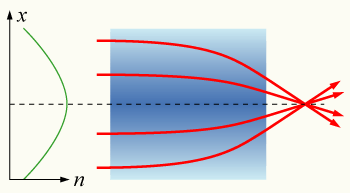
\includegraphics[width=0.4\textwidth]{Grin-lens.png}
\end{figure}
Una lente GRIN tagliata a $\lambda/4$ focalizza assi parassiali sulla superficie e viceversa. La lente GRIN a nostra disposizione � tagliata a 0.29$\lambda$ quindi focalizza onde sferiche ad una certa distanza dalla superficie.

\subsection{Coefficiente di accoppiamento}
L'idea � usare la lente GRIN per lanciare luce in fibra. Misuriamo quindi il coefficiente di accoppiamento di una sorgente laser o LED a una fibra ottica multimodo attraverso una lente GRIN.
Il coefficiente di accoppiamento si ottiene con la formula
\[\Gamma = 10 \log\left |\frac{P_{in}}{P_{out}} \right|\] 
dove $P_{in}$ � la potenza in ingresso, misurata con il \textit{power meter} a diretto contatto con la sorgente, e $P_{out}$ � la potenza in uscita, misurata, con lo stesso \textit{power meter}, all'uscita della fibra ottica.

\begin{table}[H]
	\centering
	\begin{tabular}{|c|cccc|}
		\hline
		& $I_{in}$ [mA]  & $P_{in}$ [mW]& $P_{out}$ [mW]& $\Gamma [dB]$ \\
		\hline
		laser  & 78.0(1) & 6.19(6) & 3.50(1) & 2.48(4)\\

		LED & 81.1(2) & 8.21(10) & 0.00491(2) & 32.23(6)\\
		\hline
	\end{tabular}
\end{table}



\subsection{Trasmissione di un segnale}

\end{multicols}
	
\end{document}